\section{Results}
\label{sec:results}

\subsection{Kiara Versus Lucene (S1)}
\label{sec:lucene}
Table~\ref{tab:lucene} reports the in-process comparison. Kiara had lower aggregate latency on equivalent structured queries for all five datasets, from 3.46$\times$ on the 100,000-event schedule to 16.07$\times$ on the 10,000-product catalog. For keyword scenarios that returned equivalent results in every fork, the corresponding ratios were 2.15--6.05$\times$. The aggregates weight each query equally, and Kiara did not win every individual query. The suite recorded 738 scenario--fork measurements and 37,110 samples, and all 30 worker builds succeeded.

The cost is on the build side. At 10,000 records, build times were similar. At 100,000 records, Lucene built its index 38$\times$ (catalog) and 26$\times$ (schedule) faster. Lucene also retained 11--20$\times$ less additional heap, measured as post-build heap growth after requested garbage collection. As Section~\ref{sec:cost} predicts, Kiara's build cost under the shared unique-first schema is quadratic. Unique-first placement also removes prefix sharing, so the memory figures represent an unfavorable layout for Kiara rather than its best case.

\begin{table}[t]
\centering
\caption{Kiara Versus Lucene (S1): Aggregate Lucene/Kiara Latency Ratios, Build Time, and Additional Retained Heap}
\label{tab:lucene}
\setlength{\tabcolsep}{2pt}
\begin{tabular}{@{}lrrrcc@{}}
\toprule
Dataset & Eq. & Struct. & Kw. & Build s (K/L) & Heap MiB (K/L) \\
\midrule
retail 3,788 & 5 & 7.98 & 2.15 & 0.49/0.67 & 14.1/0.7 \\
catalog 10k & 22 & 16.07 & 6.05 & 1.15/1.12 & 33.5/2.1 \\
catalog 100k & 22 & 9.43 & 4.63 & 183.0/4.76 & 327.4/20.0 \\
schedule 10k & 22 & 5.42 & -- & 1.30/1.46 & 33.4/2.9 \\
schedule 100k & 22 & 3.46 & -- & 157.6/6.00 & 294.4/27.0 \\
\bottomrule
\multicolumn{6}{@{}p{0.95\columnwidth}@{}}{\footnotesize Eq.: equivalent structured scenarios; Kw.: equivalent-keyword ratio. Schedule fixtures contain no keyword workloads.}
\end{tabular}
\end{table}

\subsection{Kiara Versus SQL Engines (S2--S6)}
Table~\ref{tab:sql} summarizes the five SQL configurations. Three patterns stand out.

\emph{First, the timing boundary matters as much as the engine.} In the client--server configuration (S2), Kiara had 2.86--67.64$\times$ lower aggregate latency. Removing transport and client decoding (S3) moved the 100,000-record aggregates in VoltDB's favor (0.80 and 0.92). A comparison between an embedded library and a server therefore depends on whether the application actually pays network costs.

\emph{Second, generic physical design favors Kiara.} Against generic-index configurations (S4, S6), Kiara had lower aggregate latency in eleven of twelve dataset entries. The exception was the 100,000-event schedule against SQLite (0.94). On generic SQLite, Kiara also completed two queries that SQLite could not finish within the 60\,s deadline in any trial, \texttt{tags-exclude} on the large catalog and \texttt{range-list-point} on the large schedule. These outcomes are counted separately and are not converted into latencies.

\emph{Third, workload-specific tuning reverses the large-dataset results.} Tuned SQLite reached 0.30--0.69 on three of five datasets and tuned VoltDB 0.80--0.99 on three. Kiara nevertheless retained more lower per-query medians than either tuned engine on most fixtures. Against tuned VoltDB, Kiara had lower medians on 46 of 89 dataset--query pairs and VoltDB on 43. Against tuned SQLite the count was 54 of 89 for Kiara and 35 for SQLite. The aggregates are dominated by the \emph{magnitude} of a few losses, which Section~\ref{sec:anatomy} examines.

\begin{table*}[t]
\centering
\caption{Aggregate Opponent/Kiara Latency Ratios Against SQL Engines (Geometric Means; Exploratory 95\% Bootstrap Intervals in Parentheses). Values Above 1 Favor Kiara}
\label{tab:sql}
\setlength{\tabcolsep}{4pt}
\renewcommand{\arraystretch}{1.1}
\begin{tabular}{@{}lrrrrrr@{}}
\toprule
Dataset & Queries & S5 SQLite tuned & S6 SQLite generic & S3 VoltDB tuned & S4 VoltDB generic & S2 VoltDB client--server \\
\midrule
retail 3,788 & 5 & 5.30 (4.83--6.47) & 11.57 (8.52--12.65) & 10.95 (8.98--12.46) & 28.60 (21.92--31.88) & 67.64 \\
catalog 10k & 21 & 1.68 (1.43--1.74) & 3.33 (3.15--3.52) & 0.99 (0.89--1.13) & 1.52 (1.38--1.62) & 8.16 \\
catalog 100k & 21 & 0.61 (0.54--0.68) & 1.76 (1.59--1.83)$^{\ast}$ & 0.80 (0.71--0.86) & 1.14 (1.07--1.27) & 2.86 \\
schedule 10k & 21 & 0.69 (0.65--0.73) & 2.02 (1.94--2.09) & 1.32 (1.23--1.47) & 2.45 (2.30--2.60) & 10.88 \\
schedule 100k & 21 & 0.30 (0.29--0.31) & 0.94 (0.85--0.97)$^{\ast}$ & 0.92 (0.85--0.99) & 1.89 (1.75--2.00) & 4.66 \\
wide 10k & 39 & -- & -- & -- & 15.43 (15.06--16.79) & -- \\
wide 100k & 39 & -- & -- & -- & 10.99 (10.49--11.34) & -- \\
\bottomrule
\end{tabular}
\par\vspace{1mm}\parbox{0.97\textwidth}{\footnotesize $^{\ast}$20 fully measured queries; the remaining query was a deadline-completion win for Kiara. S2 used three forks and reported no intervals, and its equivalent-query sets were 5/22/22/22/22. S2 build times (Kiara/VoltDB) were 0.45/6.92\,s, 1.21/8.98\,s, 177.2/48.7\,s, 1.50/8.42\,s, and 169.6/46.5\,s in the order listed.}
\end{table*}

\subsection{Anatomy of the Extremes}
\label{sec:anatomy}
Table~\ref{tab:anatomy} lists representative 100,000-record queries against tuned VoltDB, together with the prediction from Section~\ref{sec:predictions} that accounts for each. The VoltDB plans used compound indexes, bounded index scans, and indexed set differences.

\emph{Collection membership (P1).} Queries over tags, sizes, date lists, and timestamp lists, and point-in-interval queries over stored durations, ran 16.8--70.5$\times$ faster in Kiara. On the retail fixture, ``markets contain both values'' ran 33.3$\times$ faster and ``markets exclude a value'' 25.2$\times$ faster. The relational formulations must join child rows and then group, deduplicate, or apply conditional aggregation. An index does not remove that work. Kiara intersects two short posting lists at one level.

\emph{High-fan-out predicates paired with broad ones (P2).} The worst result, ``active status and tags exclude clearance,'' took 14.2\,s in Kiara against 0.21\,s in VoltDB, and was consistent across trials (13.4--17.7\,s). \op{NOT\_CONTAINS} enumerates every distinct tag collection, which yields thousands of lists. The status predicate sits higher in the trie and matches most records, so \textsc{ExpandDown} performs one binary search per pair of status node and tag list, as Eq.~\eqref{eq:expanddown} predicts. The season query (8.8\,s against 45\,ms) has the same structure, because a stabbing query over many distinct season intervals meets a broad event-type predicate. On the small retail fixture the same operator was a strength, because neither side was large. Exclusion is therefore not intrinsically slow in Kiara. Its cost depends on the fan-out and on what it is paired with.

\emph{Same-attribute windows (P3).} The four-hour timestamp window returned 77 events. Kiara took 30.3\,ms, because two broad comparisons on a high-cardinality attribute were each materialized as candidate collections and then intersected. VoltDB took 40\,\textmu s with one bounded index scan. Kiara's \op{BETWEEN} operator generates only the qualifying keys. The benchmark fixed the two-predicate form in advance, so this ratio applies to that formulation.

\emph{Broad scalar conjunctions (P4).} ``Status and region and brand'' took 6.5\,ms in Kiara and 0.13\,ms in VoltDB, which sought a compound index on (brand, status, region, id). This is precisely the access path that Proposition~\ref{prop:indexcount} shows cannot exist for \emph{every} combination. For a fixed, known combination, however, it wins decisively.

\emph{Limits (P5).} ``First 20 active products'' took 39.8\,ms in Kiara against 27\,\textmu s in tuned SQLite (S5), which stops scanning after 20 rows. Limited queries were excluded from the ratios because no ordering contract defines a unique answer.

\begin{table}[t]
\centering
\caption{Representative 100k-Record Queries Against Tuned VoltDB (S3), Median p50 Execution Time}
\label{tab:anatomy}
\setlength{\tabcolsep}{1.8pt}
\begin{tabular}{@{}lrrrc@{}}
\toprule
Query & Kiara ms & VoltDB ms & V/K & Pred. \\
\midrule
Tags contain both values & 0.764 & 48.640 & 63.7 & P1 \\
Sizes contain both $\wedge$ category & 2.448 & 42.148 & 17.2 & P1 \\
Date list contains both & 0.251 & 15.945 & 63.6 & P1 \\
Timestamp list contains both & 0.258 & 18.180 & 70.5 & P1 \\
Duration $\ni$ point $\wedge$ city & 13.146 & 221.463 & 16.8 & P1 \\
Brand equality & 0.549 & 0.553 & 1.01 & -- \\
Status $\ne$ archived & 48.026 & 20.680 & 0.43 & P2 \\
Active $\wedge$ tags exclude & 14{,}241 & 210.456 & 0.015 & P2 \\
Season $\ni$ date $\wedge$ type & 8{,}843 & 45.275 & 0.0051 & P2 \\
Four-field conjunction & 391.368 & 3.101 & 0.0079 & P2, P4 \\
Timestamp 4-hour window & 30.256 & 0.040 & 0.0013 & P3 \\
Status $\wedge$ region $\wedge$ brand & 6.544 & 0.132 & 0.020 & P4 \\
\bottomrule
\end{tabular}
\end{table}

\subsection{Wide Filters (S7)}
Fig.~\ref{fig:wide} plots the 100,000-record collection families against attribute width. Four results stand out.
\begin{enumerate}
\item With two attributes, Kiara had lower latency than every opponent in the \op{CONTAINS\_EITHER} family, and than every opponent except tuned SQLite (0.61) in the \op{CONTAINS\_ALL} family. Against generic SQLite, the advantage was 25--80$\times$.
\item As width grew to eight or more attributes, tuned SQLite and Lucene overtook Kiara, reaching opponent/Kiara ratios of 0.02--0.16.
\item Against tuned VoltDB, Kiara remained faster at \emph{every} collection width, by 1.26--13.9$\times$ for \op{CONTAINS\_EITHER} and 1.37--12.5$\times$ for \op{CONTAINS\_ALL}.
\item Generic SQLite degraded sharply at 12--16 attributes. Where it completed, it was 298--408$\times$ slower than Kiara. It exceeded the 60\,s deadline in all trials of 9 of the 12 wide-100k queries at those widths, and Kiara completed every one.
\end{enumerate}
The 10,000-record results follow the same pattern.

The scalar-only family isolates prediction P4. At two attributes Kiara was faster than VoltDB (21$\times$), generic SQLite (34$\times$), and Lucene (12$\times$), and essentially tied with tuned SQLite (0.96). At four and eight attributes every opponent was faster. Tuned SQLite was faster by 77--200$\times$, using a covering index whose leading column is the selective attribute. Kiara's own latency also rose sharply between widths four and eight. For example, \op{CONTAINS\_EITHER} at 1\% selectivity on 10,000 records rose from 0.13\,ms to 3.3\,ms as broad predicates entered shallow levels. This behavior is consistent with level-ordered rather than selectivity-ordered evaluation.

\begin{figure*}[t]
\centering
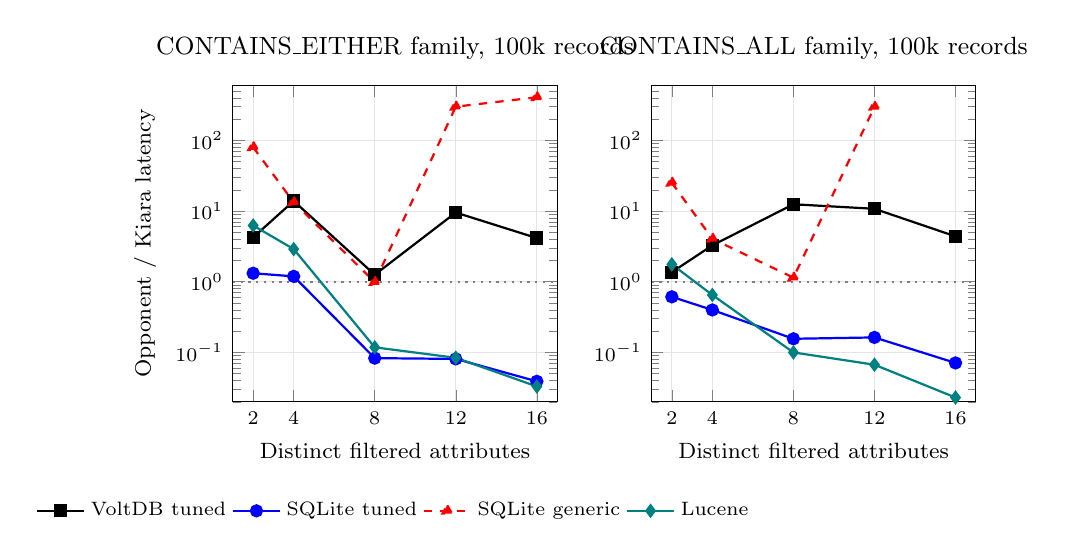
\begin{tikzpicture}
\begin{axis}[
  name=either, width=0.47\textwidth, height=5.6cm,
  ymode=log, ymin=0.02, ymax=600,
  xtick={2,4,8,12,16}, xmin=1, xmax=17,
  xlabel={Distinct filtered attributes}, ylabel={Opponent / Kiara latency},
  title={\small \op{CONTAINS\_EITHER} family, 100k records},
  tick label style={font=\scriptsize}, label style={font=\footnotesize},
  legend style={font=\scriptsize, at={(0.5,-0.28)}, anchor=north, legend columns=4, draw=none},
  grid=major, grid style={gray!20}]
\addplot[black, mark=square*, thick] coordinates {(2,4.246) (4,13.905) (8,1.257) (12,9.535) (16,4.151)};
\addplot[blue, mark=*, thick] coordinates {(2,1.319) (4,1.192) (8,0.083) (12,0.081) (16,0.039)};
\addplot[red, mark=triangle*, thick, dashed] coordinates {(2,80.115) (4,13.329) (8,0.990) (12,300.158) (16,407.571)};
\addplot[teal, mark=diamond*, thick] coordinates {(2,6.257) (4,2.898) (8,0.118) (12,0.084) (16,0.033)};
\addplot[gray, dotted, thick, forget plot] coordinates {(1,1) (17,1)};
\legend{VoltDB tuned, SQLite tuned, SQLite generic, Lucene}
\end{axis}
\begin{axis}[
  at={(either.east)}, anchor=west, xshift=12mm,
  width=0.47\textwidth, height=5.6cm,
  ymode=log, ymin=0.02, ymax=600,
  xtick={2,4,8,12,16}, xmin=1, xmax=17,
  xlabel={Distinct filtered attributes},
  title={\small \op{CONTAINS\_ALL} family, 100k records},
  tick label style={font=\scriptsize}, label style={font=\footnotesize},
  grid=major, grid style={gray!20}]
\addplot[black, mark=square*, thick] coordinates {(2,1.366) (4,3.275) (8,12.489) (12,10.773) (16,4.386)};
\addplot[blue, mark=*, thick] coordinates {(2,0.612) (4,0.399) (8,0.156) (12,0.163) (16,0.071)};
\addplot[red, mark=triangle*, thick, dashed] coordinates {(2,25.183) (4,4.058) (8,1.142) (12,298.414)};
\addplot[teal, mark=diamond*, thick] coordinates {(2,1.763) (4,0.650) (8,0.100) (12,0.067) (16,0.023)};
\addplot[gray, dotted, thick, forget plot] coordinates {(1,1) (17,1)};
\end{axis}
\end{tikzpicture}
\caption{Wide-filter results (S7) for 100,000 records: geometric-mean opponent/Kiara latency over three selectivity targets. Values above the dotted line favor Kiara. Generic-SQLite points at width 12 (both families) and width 16 (\op{CONTAINS\_EITHER}) are based on the one target that completed in every trial; the other targets exceeded the 60\,s deadline in every trial. Generic SQLite timed out on every \op{CONTAINS\_ALL} query at width 16, which therefore has no point. Kiara completed all queries.}
\label{fig:wide}
\end{figure*}

\subsection{Correctness Findings}
\label{sec:correctness}
The oracle uncovered four behaviors that a latency-only benchmark would have hidden.
\begin{enumerate}
\item \emph{Fractional truncation.} Because numeric keys are truncated to integers, \texttt{price < 0.20} returned none of 121 expected products, \texttt{price <= 19.50} also matched 19.99, and \texttt{price = 19.99} matched 209 products instead of 3 on the large catalog. Forty scenario--trial entries were excluded on this basis in each five-trial base suite (S3--S6).
\item \emph{Cross-attribute normalization.} The retail fixture indexes raw title tokens in one attribute and stemmed tokens in another. For the query \emph{lanterns}, Kiara returned 18 records, while Lucene and the oracle returned 20, including plural titles. Kiara keeps a single normalized form per keyword across all attributes the keyword binds to (Section~\ref{sec:text}). Keeping one form per bound attribute would correct this implementation limitation.
\item \emph{Interval comparator contract.} Version 2.0.15 failed to build the realistic schedule indexes. The defect was diagnosed and fixed in 2.0.16 (Section~\ref{sec:system}), and all builds subsequently succeeded.
\item \emph{Limits.} Different engines returned different valid subsets for limited queries. Applications that need deterministic pagination must impose an order.
\end{enumerate}
